\section{Présentation de l'entreprise}
\subsection{Sopra Steria}
En 2014 le Sopra Group fusionne avec l'entreprise Steria, deux très grandes entreprises dans le domaine des systèmes d'informations, Sopra Steria est un acteur majeur de la transformation numérique en Europe.
\textit{ Sopra Steria propose des prestations de conseil et des services technologiques (intégration de systèmes, gestion d’infrastructures, exécution de processus métier) et est un éditeur de logiciels métier (RH, banque, immobilier). L'entreprise compte plus de 37 000 collaborateurs et est présente à travers plus de vingt pays. Elle est surtout présente et reconnue en Europe notamment en France et en Angleterre où elle réalise la majeure partie de son chiffre d'affaire}.\\

Grâce à ses différentes filiales, Sopra Steria est présent sur de nombreux secteurs ainsi que dans de nombreux domaines :\\
\begin{figure}[h]
\centering
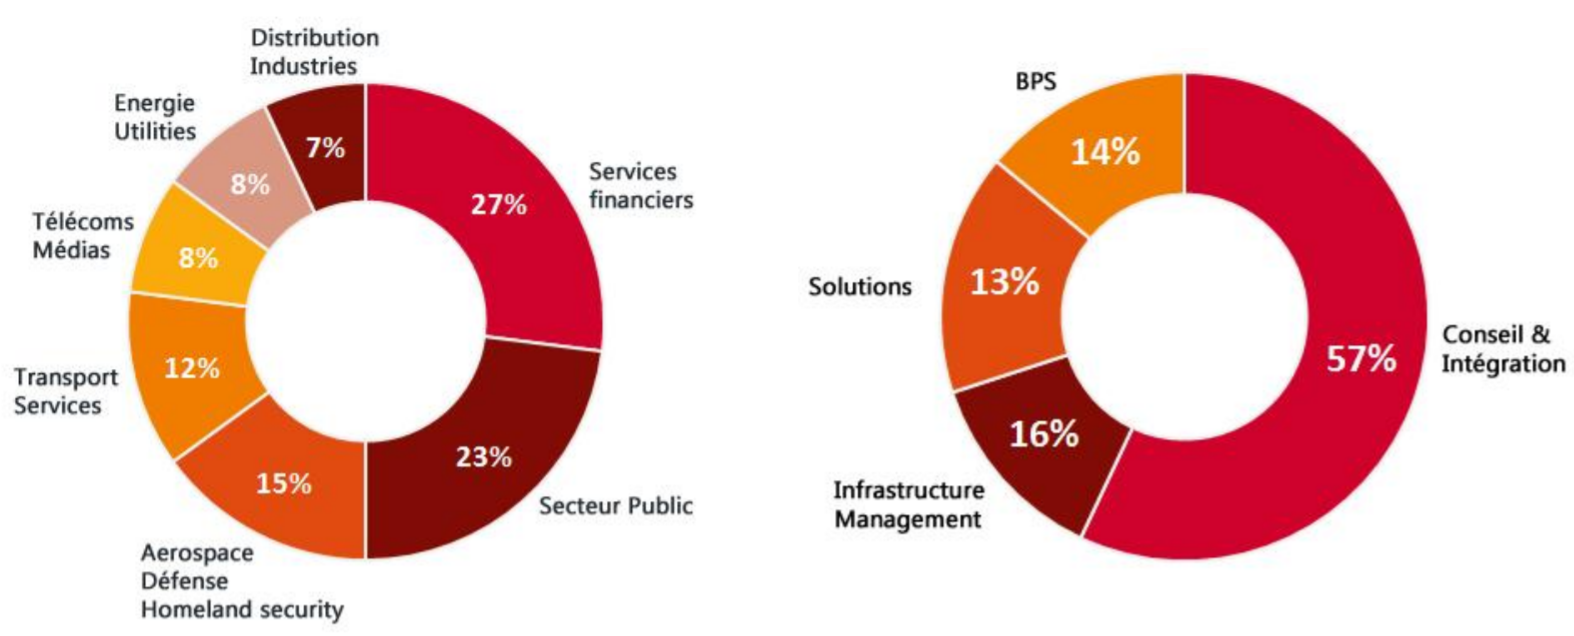
\includegraphics[scale=0.6]{resources/sopraSteriaGraph.png}
\caption{Secteurs et domaines d'activités de Sopra Steria}
\label{sopraSteriaGraph}
\end{figure}

Pour ma part, j'ai travaillé pour la filiale Sopra Banking Software.

\newpage
\subsection{Sopra Banking Software}
\textit{La transformation numérique entraîne un véritable bouleversement dans les organisations et les modes de travail, dans les pratiques managériales et dans l’engagement des collaborateurs.}\\

\textit{Sopra Banking Software est une filiale du groupe Sopra Steria, leader européen de la transformation numérique. Avec plus de 44 000 collaborateurs, ce dernier affiche un chiffre d’affaires 2018 de 4,1 milliard d’euros.}\\

\textit{Avec ses 4000 experts, un chiffre d’affaires 2018 de 373,7 millions d’euros et l’un des portefeuilles de solutions et de services les plus complets du marché, Sopra Banking Software est de longue date le partenaire de confiance de plus de 800 banques dans 70 pays.}\\

\textit{Son savoir-faire sans égal lui permet de répondre aux besoins d’innovation comme de développement de banques et institutions financières de toute taille et activité.\footnote{Source dans la webographie}}\\

Sopra Banking Software propose des solutions financières à destination des banques et des instituions financières. Elle est présente en Europe, Asie, Afrique et depuis peu en Amérique du nord. 


\begin{figure}[h]
\centering
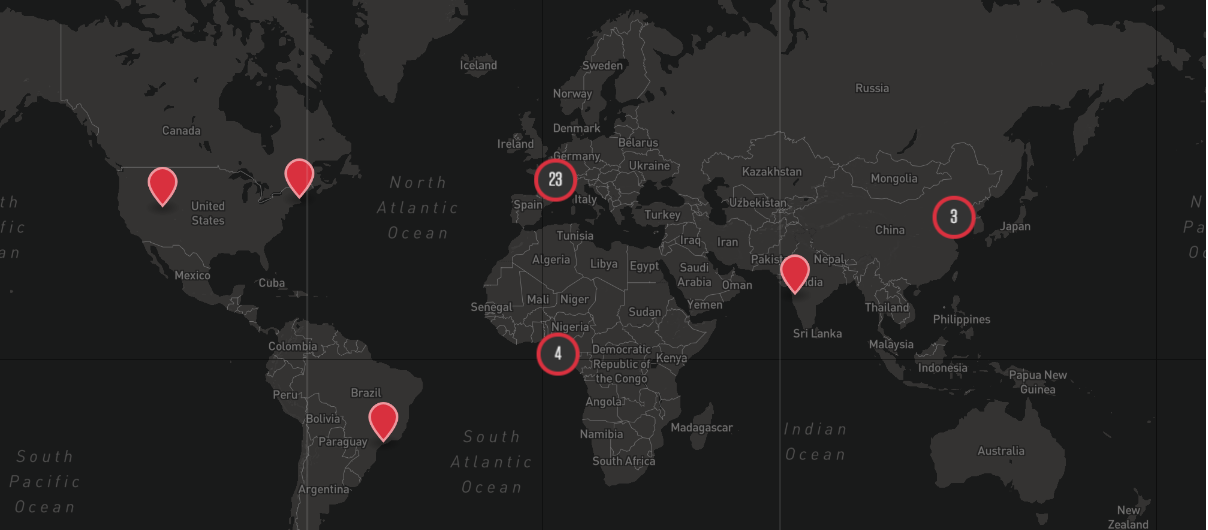
\includegraphics[scale=0.6]{resources/SBSImplantSites.png}
\caption{Implantation \& sites de Sopra Banking Software}
\label{SBSImplantSites}
\end{figure}

\newpage
\subsection{O.R. System}

\textit{O.R. System est un fournisseur de solutions et logiciels pour la gestion du risque de contrepartie, l’analyse financière et la notation interne. Avec plus de 300 000 utilisateurs dans 70 pays, nous sommes leaders sur notre marché. Nous nous engageons à agir comme partenaire pour chacun de nos clients, à créer de la valeur pour eux, et nous nous adaptons constamment à leurs marchés et besoins.}\\

\textit{Afin d’accompagner ses clients O.R. System a une équipe de spécialistes multidisciplinaires : experts métiers (analyse financière et notation), chefs de projets, experts produits, architectes techniques, et formateurs.
Créée en 1985, O.R. System débuta en tant qu’éditeur de logiciel dédié aux banques et institutions financières.
La première version de son produit phare ANADEFI fut développée et implémentée au début des années 90 : un outil puissant d’analyse financière afin d’aider les institutions financières à évaluer leurs clients et contreparties.}\\

\textit{Avec le développement rapide des réglementations Bâle I et II, d’un pur outil financier ANADEFI s’est transformé en plateforme complète supportant l’implémentation de toute méthode de notation interne.}\\

\textit{En 2005, O.R. System lance une version d’ANADEFI dédiée aux Banques Centrales leur fournissant une solution complète pour la gestion de leurs informations financières, et de leurs bases de données risques et incidents de paiement.}\\

\textit{Sopra Banking Software rachete O.R System en 2019.
Cette acquisition permet à la nouvelle équipe de donner un nouveau départ à l’entreprise et d’accélérer sa croissance, en France comme à l’international.
L’un des objectifs de la nouvelle direction est de développer ses parts de marché à l’international et de nouvelles offres dans le domaine de la gestion de risques de contrepartie.\footnote{Source dans la webographie}}\\

Sur le plan organisationnel, le siège social est désormais à la tour Manhattan située à la Défense mais elle conserve les équipes techniques et administratives sur Montpellier. Plusieurs agences\footnote{Les équipes de Sopra Banking Software sont reparties par agence.} vont s'occuper des différents pôles d'Anadefi.


